\documentclass[a4paper,10pt]{ltjsarticle}

% 各種字体
% cf. http://www.yamamo10.jp/yamamoto/comp/latex/make_doc/formula/amsmath_symbol/index.php
\usepackage{amsmath,amssymb,amsfonts}

% 定番スニペット
% cf. https://mirrors.ctan.org/macros/latex/contrib/physics2/physics2.pdf
\usepackage{physics2}
% automatic braces
\usephysicsmodule{ab}

% 単位
% cf. http://www.yamamo10.jp/yamamoto/comp/latex/make_doc/unit/index.php
\usepackage{siunitx}

% 画像挿入
\usepackage{graphicx}
% ハイパーリンク, URL 挿入
\usepackage{hyperref,url}

% 改ページできるフレーム
\usepackage{framed}
% 色付き文字
\usepackage{xcolor}

%---------------%
% 適宜切り替える %
%---------------%

% 、。と ,. の切り替え (LuaLaTeX 専用)
\usepackage{newunicodechar}
\newunicodechar{、}{,}
\newunicodechar{。}{.}

% ページ数を消す
% \pagestyle{empty}

\begin{document}

\section{サンプル}

\LaTeX。
% 助詞の連続のエラー例
textlint で文法ががェックできます。
% である・ですます のエラー例
本日はは晴天である。
AdS/CFT~\cite{maldacena1999large}
の概要を図~\ref{fig:adscft}に示します。

\begin{figure}[tbp]
  \begin{center}
    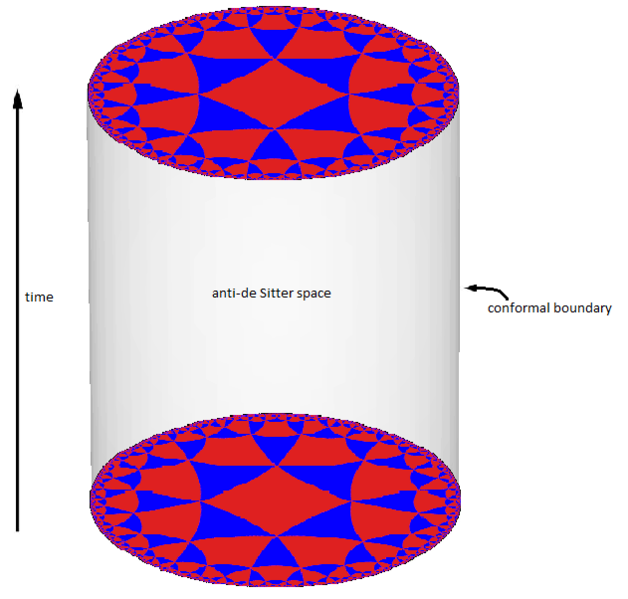
\includegraphics[width=8cm]{img/sample.png}
    \caption{AdS/CFT対応の概念図~\cite{adscftwiki}}
  \end{center}
  \label{fig:adscft}
\end{figure}

\bibliography{reference}
% 掲載順=引用順
% cf. https://mathlandscape.com/latex-bibstyles/
\bibliographystyle{unsrt}

\end{document}